{\color{indiagreen}\subsection{Premo gibanje}}
\textbf{Premik} definiramo kot \underline{razdaljo} med \underline{začetno} in \underline{kočno lego}, kateremu lahko določimo smer.(se vprašamo kam)\\
\textbf{Zapis}:
\\
Kartezični(Vektor) $\rightarrow$ \quad $(-60 km, -70 km)$ ali $(x, y)$\\
Cilindrične kordinate $\rightarrow$ \quad $(-92 km, 230 \,^{\circ}\mathrm{C})$ ali $(r, \alpha)$\\
\\
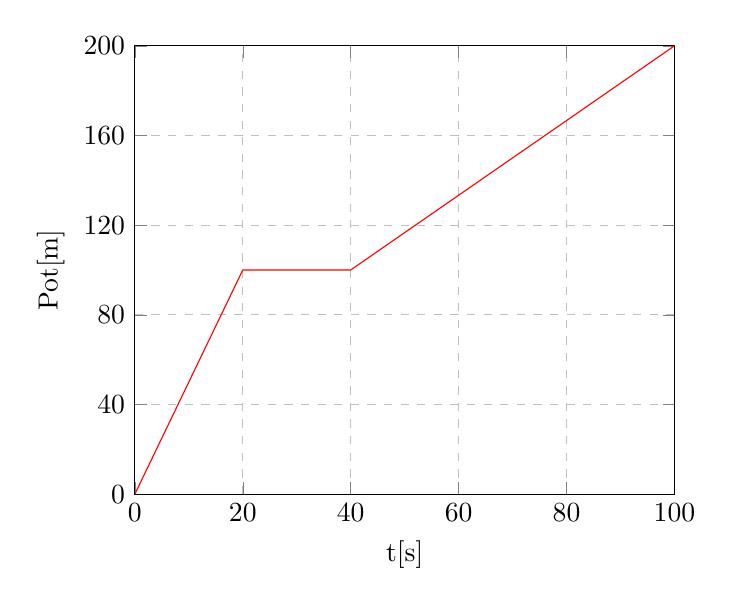
\begin{tikzpicture}
\begin{axis}[
    xlabel={t[s]},
    ylabel={Pot[m]},
    xmin=0, xmax=100,
    ymin=0, ymax=200,
    xtick={0,20,40,60,80,100},
    ytick={0,40,80,120,160,200},
    ymajorgrids=true,
    xmajorgrids=true,
    grid style=dashed,
]
 
\addplot[
    color=red,
    ]
    coordinates {

    (0,0)(20,100)(40,100)(100,200)
    };
 
\end{axis}
\end{tikzpicture}

Pot se vedno \textbf{veča} zato nikoli ne gre v \textbf{minus}.